
\chapter{Sprint 3 : Planning intelligent et assistant d'apprentissage}
\label{chap:sprint3}

\section{Introduction}
\addcontentsline{toc}{section}{Introduction}

Le troisième sprint constitue une étape clé dans le développement du système \textit{Smart Focus}. Il porte sur l'intégration des modules d'intelligence artificielle destinés à accompagner l'utilisateur dans l'organisation de ses sessions d'étude et dans l'exploitation de ses ressources pédagogiques.

Ce sprint couvre le développement du système de planification intelligent, capable de générer automatiquement des sessions d'étude adaptées au profil de l'utilisateur et à son état de sommeil. Il intègre également le chatbot RAG permettant d'interroger des documents PDF, ainsi que les modules de génération de quiz QCM et de flashcards avec révision espacée basée sur l'algorithme SM-2.

Enfin, ce sprint assure la connexion des interfaces mobiles aux données dynamiques du backend, permettant une interaction fluide entre l'utilisateur et les fonctionnalités intelligentes du système.

\section{Backlog du Sprint 3}

Le backlog du Sprint 3 regroupe les fonctionnalités liées à l'intelligence artificielle et à l'assistance pédagogique. Ces éléments représentent le cœur applicatif du système, combinant la planification adaptative, l'exploitation documentaire et les outils de révision.

Chaque fonctionnalité est formulée sous forme de \textit{User Stories}, permettant de décrire les attentes des utilisateurs tout en orientant les tâches de développement. Le tableau~\ref{tab:backlogs3} présente le backlog détaillé du troisième sprint.

\begin{table}[H]
\centering
\renewcommand{\arraystretch}{1.3}
\begin{tabular}{|c|p{3cm}|p{6cm}|p{4cm}|}
\hline
\textbf{ID} & \textbf{Fonctionnalité} & \textbf{User Story} & \textbf{Tâche} \\
\hline

US9 & Chatbot intelligent (RAG)
& En tant qu'utilisateur, je souhaite interagir avec un chatbot pour poser des questions et réviser mes cours
& Implémentation du pipeline RAG : chunking, embeddings, recherche sémantique et génération contextuelle via Groq \\ \hline

US10 & Import de documents
& En tant qu'utilisateur, je souhaite importer mes cours au format PDF afin qu'ils soient utilisés par le chatbot
& Développement de l'upload PDF avec extraction via PyMuPDF, stockage dans ChromaDB et validation CSV \\ \hline

US11 & Génération de quiz et flashcards
& En tant qu'utilisateur, je souhaite générer des quiz QCM et des flashcards pour tester mes connaissances
& Implémentation des générateurs IA avec prompts Groq, validation JSON et algorithme SM-2 \\ \hline

US12 & Planification intelligente
& En tant qu'utilisateur, je souhaite obtenir un planning de révision adapté à mon profil et à mon sommeil
& Développement du calcul déterministe des créneaux libres avec assignation IA des sujets via Groq \\ \hline

\end{tabular}
\caption{Backlog du Sprint 3}
\label{tab:backlogs3}
\end{table}

\section{Spécifications fonctionnelles}

\subsection{Diagramme de cas d'utilisation du Sprint 3}

Le diagramme de cas d'utilisation suivant illustre les principales interactions entre l'utilisateur et le système durant le troisième sprint, couvrant les fonctionnalités liées au chatbot RAG, à la génération de quiz et flashcards, ainsi qu'à la planification intelligente.

\begin{figure}[H]
\centering
\includegraphics[width=1\textwidth]{images/usecasesprint3.jpg}
\caption{Diagramme de cas d'utilisation du Sprint 3}
\end{figure}

%%%%%%%%%%%%%%%%%%%%%%%%%%%%%%%%%%%%%%%%%%%%%%%%%%%%%%%%%%%

\subsection{Description textuelle des cas d'utilisation}

Afin de mieux expliciter le comportement du système, les cas d'utilisation du troisième sprint sont présentés sous forme de fiches descriptives. Chaque tableau synthétise les interactions entre l'utilisateur et le système, en mettant en évidence les étapes principales ainsi que les conditions de déroulement.

%----------------------------------------
\subsubsection{Cas d'utilisation : Uploader un document}

L'import de documents constitue le point d'entrée du pipeline RAG. Ce processus permet à l'utilisateur de télécharger un fichier PDF qui sera découpé en chunks, vectorisé puis indexé dans ChromaDB pour une exploitation ultérieure. Le Tableau~\ref{tab:uc_upload} présente les différentes étapes de ce processus.

\begin{table}[H]
\centering
\renewcommand{\arraystretch}{1.2}
\begin{tabular}{|p{4cm}|p{10cm}|}
\hline
\textbf{Acteur} & Utilisateur \\ \hline

\textbf{Objectif} & Importer un document PDF pour l'exploiter via le chatbot, les quiz et les flashcards \\ \hline

\textbf{Conditions initiales} & Utilisateur authentifié, fichier PDF ou CSV valide \\ \hline

\textbf{Déroulement} &
\begin{itemize}
    \item Sélection du fichier depuis l'interface mobile
    \item Envoi du fichier au backend via l'API d'upload
    \item Extraction du texte par page via PyMuPDF
    \item Découpage en chunks via RecursiveCharacterTextSplitter
    \item Génération des embeddings via HuggingFace (all-MiniLM-L6-v2)
    \item Stockage des vecteurs dans ChromaDB
    \item Enregistrement des métadonnées dans PostgreSQL
\end{itemize} \\ \hline

\textbf{Cas d'erreur} & Fichier vide ou sans texte extractible → rejet avec message d'erreur \\ \hline

\textbf{Résultat} & Document indexé et prêt pour la recherche sémantique \\ \hline
\end{tabular}
\caption{Description du cas d'utilisation « Uploader un document »}
\label{tab:uc_upload}
\end{table}

%----------------------------------------
\subsubsection{Cas d'utilisation : Poser une question RAG}

Le chatbot RAG permet à l'utilisateur de poser des questions sur le contenu de ses documents importés. Le système effectue une recherche sémantique dans ChromaDB puis construit un prompt contextuel envoyé à Groq pour générer une réponse précise. Le Tableau~\ref{tab:uc_rag_chat} détaille ce processus.

\begin{table}[H]
\centering
\renewcommand{\arraystretch}{1.2}
\begin{tabular}{|p{4cm}|p{10cm}|}
\hline
\textbf{Acteur} & Utilisateur \\ \hline

\textbf{Objectif} & Obtenir une réponse contextuelle basée sur ses documents importés \\ \hline

\textbf{Conditions initiales} & Au moins un document indexé dans ChromaDB \\ \hline

\textbf{Déroulement} &
\begin{itemize}
    \item Saisie de la question dans l'interface du chatbot
    \item Sélection des documents sources
    \item Recherche sémantique (top-k chunks par collection)
    \item Construction du contexte à partir des chunks récupérés
    \item Génération de la réponse par Groq (llama-3.3-70b-versatile)
    \item Affichage de la réponse avec citations des sources
    \item Persistance de l'échange dans la base de données
\end{itemize} \\ \hline

\textbf{Cas d'erreur} & Aucun document sélectionné → mode de réponse générale sans RAG \\ \hline

\textbf{Résultat} & Réponse contextualisée avec références aux pages sources \\ \hline
\end{tabular}
\caption{Description du cas d'utilisation « Poser une question RAG »}
\label{tab:uc_rag_chat}
\end{table}

%----------------------------------------
\subsubsection{Cas d'utilisation : Générer un quiz}

La génération de quiz permet de créer des questionnaires à choix multiples à partir du contenu des documents indexés. Le système utilise Groq pour produire des questions variées avec explications. Le Tableau~\ref{tab:uc_quiz} présente ce processus.

\begin{table}[H]
\centering
\renewcommand{\arraystretch}{1.2}
\begin{tabular}{|p{4cm}|p{10cm}|}
\hline
\textbf{Acteur} & Utilisateur \\ \hline

\textbf{Objectif} & Tester ses connaissances à travers un quiz QCM généré automatiquement \\ \hline

\textbf{Conditions initiales} & Au moins un document indexé ou une session terminée avec documents liés \\ \hline

\textbf{Déroulement} &
\begin{itemize}
    \item Sélection du ou des documents sources
    \item Choix du nombre de questions (3 à 30)
    \item Récupération et échantillonnage des chunks depuis ChromaDB
    \item Génération des questions QCM par Groq (4 options, explication)
    \item Validation de la structure JSON retournée
    \item Création du quiz en base de données
    \item Affichage des questions (réponses masquées avant soumission)
\end{itemize} \\ \hline

\textbf{Cas d'erreur} & Génération JSON invalide → rejet avec message d'erreur \\ \hline

\textbf{Résultat} & Quiz QCM prêt à être complété par l'utilisateur \\ \hline
\end{tabular}
\caption{Description du cas d'utilisation « Générer un quiz »}
\label{tab:uc_quiz}
\end{table}

%----------------------------------------
\subsubsection{Cas d'utilisation : Générer et réviser des flashcards}

Les flashcards utilisent l'algorithme de répétition espacée SM-2 pour optimiser la mémorisation à long terme. Le système génère des cartes recto/verso à partir des documents et planifie automatiquement les prochaines révisions. Le Tableau~\ref{tab:uc_flashcard} décrit ce processus.

\begin{table}[H]
\centering
\renewcommand{\arraystretch}{1.2}
\begin{tabular}{|p{4cm}|p{10cm}|}
\hline
\textbf{Acteur} & Utilisateur \\ \hline

\textbf{Objectif} & Réviser ses cours à l'aide de flashcards avec répétition espacée \\ \hline

\textbf{Conditions initiales} & Au moins un document indexé \\ \hline

\textbf{Déroulement} &
\begin{itemize}
    \item Sélection du ou des documents sources
    \item Génération des flashcards par Groq (front/back)
    \item Initialisation des paramètres SM-2 (ease\_factor = 2.5, interval = 1)
    \item Révision : l'utilisateur évalue sa qualité de rappel (0 à 5)
    \item Calcul SM-2 du prochain intervalle de révision
    \item Affichage des cartes dues (next\_review $\leq$ date actuelle)
\end{itemize} \\ \hline

\textbf{Cas d'erreur} & Aucun chunk exploitable → message d'erreur \\ \hline

\textbf{Résultat} & Deck de flashcards avec planification de révision automatique \\ \hline
\end{tabular}
\caption{Description du cas d'utilisation « Générer et réviser des flashcards »}
\label{tab:uc_flashcard}
\end{table}

%----------------------------------------
\subsubsection{Cas d'utilisation : Générer un planning intelligent}

La planification intelligente combine un calcul déterministe des créneaux libres avec une assignation des sujets par intelligence artificielle. Le planning s'adapte au profil de sommeil de l'utilisateur et à son emploi du temps. Le Tableau~\ref{tab:uc_planning} présente ce processus.

\begin{table}[H]
\centering
\renewcommand{\arraystretch}{1.2}
\begin{tabular}{|p{4cm}|p{10cm}|}
\hline
\textbf{Acteur} & Utilisateur \\ \hline

\textbf{Objectif} & Obtenir un planning de révision optimisé et adapté à son état \\ \hline

\textbf{Conditions initiales} & Utilisateur authentifié avec un profil configuré \\ \hline

\textbf{Déroulement} &
\begin{itemize}
    \item Récupération du profil sommeil et des contraintes horaires
    \item Extraction de l'emploi du temps depuis le document CSV/PDF
    \item Calcul déterministe des créneaux libres (sans chevauchement)
    \item Filtrage selon la préférence horaire (matin, après-midi, soir)
    \item Dimensionnement des sessions selon le score de sommeil
    \item Assignation des sujets de révision par Groq
    \item Fallback déterministe en cas d'échec de l'IA
    \item Persistance des sessions dans PostgreSQL
\end{itemize} \\ \hline

\textbf{Cas d'erreur} & Aucun créneau disponible → aucune session générée \\ \hline

\textbf{Résultat} & Planning journalier avec sessions adaptées au profil utilisateur \\ \hline
\end{tabular}
\caption{Description du cas d'utilisation « Générer un planning intelligent »}
\label{tab:uc_planning}
\end{table}

%%%%%%%%%%%%%%%%%%%%%%%%%%%%%%%%%%%%%%%%%%%%%%%%%%%%%%%%%%%%%%%%%%%%%%
\section{Conception}
\subsection{Diagrammes de séquence}

Afin de détailler le fonctionnement dynamique du système, les diagrammes de séquence suivants illustrent les interactions entre les différents composants pour chaque cas d'utilisation du Sprint 3.

%----------------------------------------
\subsubsection{Processus d'upload et d'indexation d'un document}

Le processus d'upload constitue la première étape du pipeline RAG. Comme illustré dans la Figure~\ref{fig:seq_upload}, le document PDF est transmis au backend qui procède à l'extraction du texte, au découpage en chunks et à la vectorisation via le modèle d'embeddings HuggingFace. Les vecteurs sont ensuite stockés dans ChromaDB tandis que les métadonnées sont persistées dans PostgreSQL.

\begin{figure}[H]
\centering
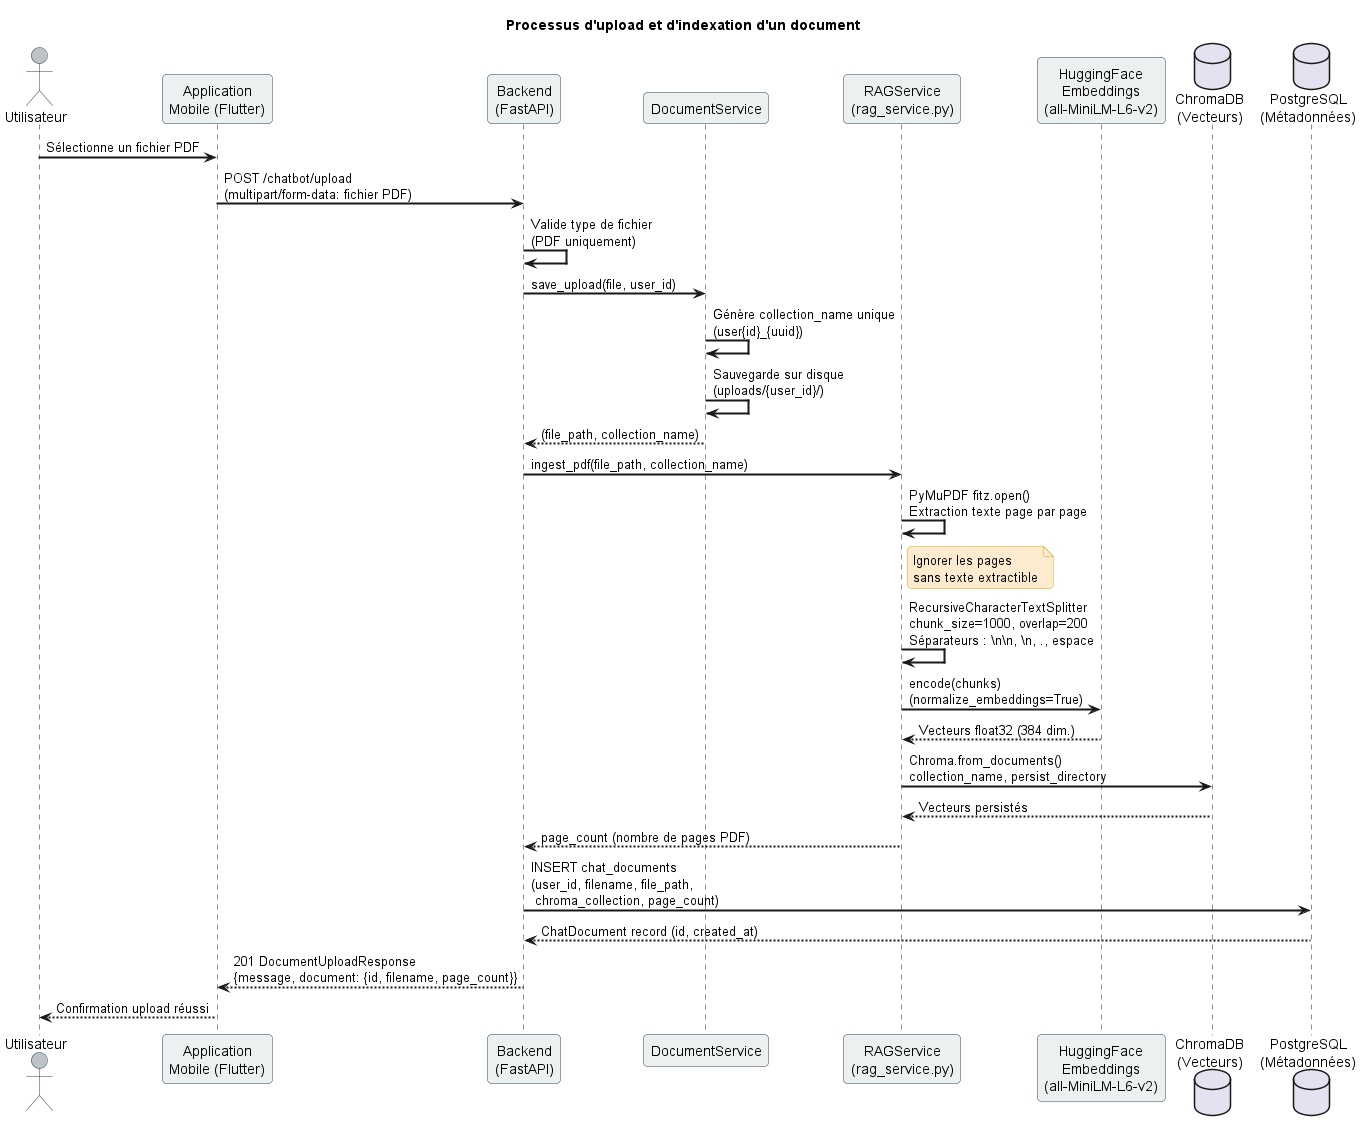
\includegraphics[width=0.85\textwidth]{images/seq_upload.jpg}
\caption{Diagramme de séquence du processus d'upload et d'indexation}
\label{fig:seq_upload}
\end{figure}

%----------------------------------------
\subsubsection{Processus de chat RAG}

Le processus de chat RAG permet à l'utilisateur d'interroger ses documents de manière contextuelle. Comme montré dans la Figure~\ref{fig:seq_chat_rag}, la question est envoyée au backend qui effectue une recherche sémantique dans ChromaDB. Les chunks les plus pertinents sont assemblés en contexte et envoyés à Groq pour générer une réponse précise accompagnée de citations.

\begin{figure}[H]
\centering
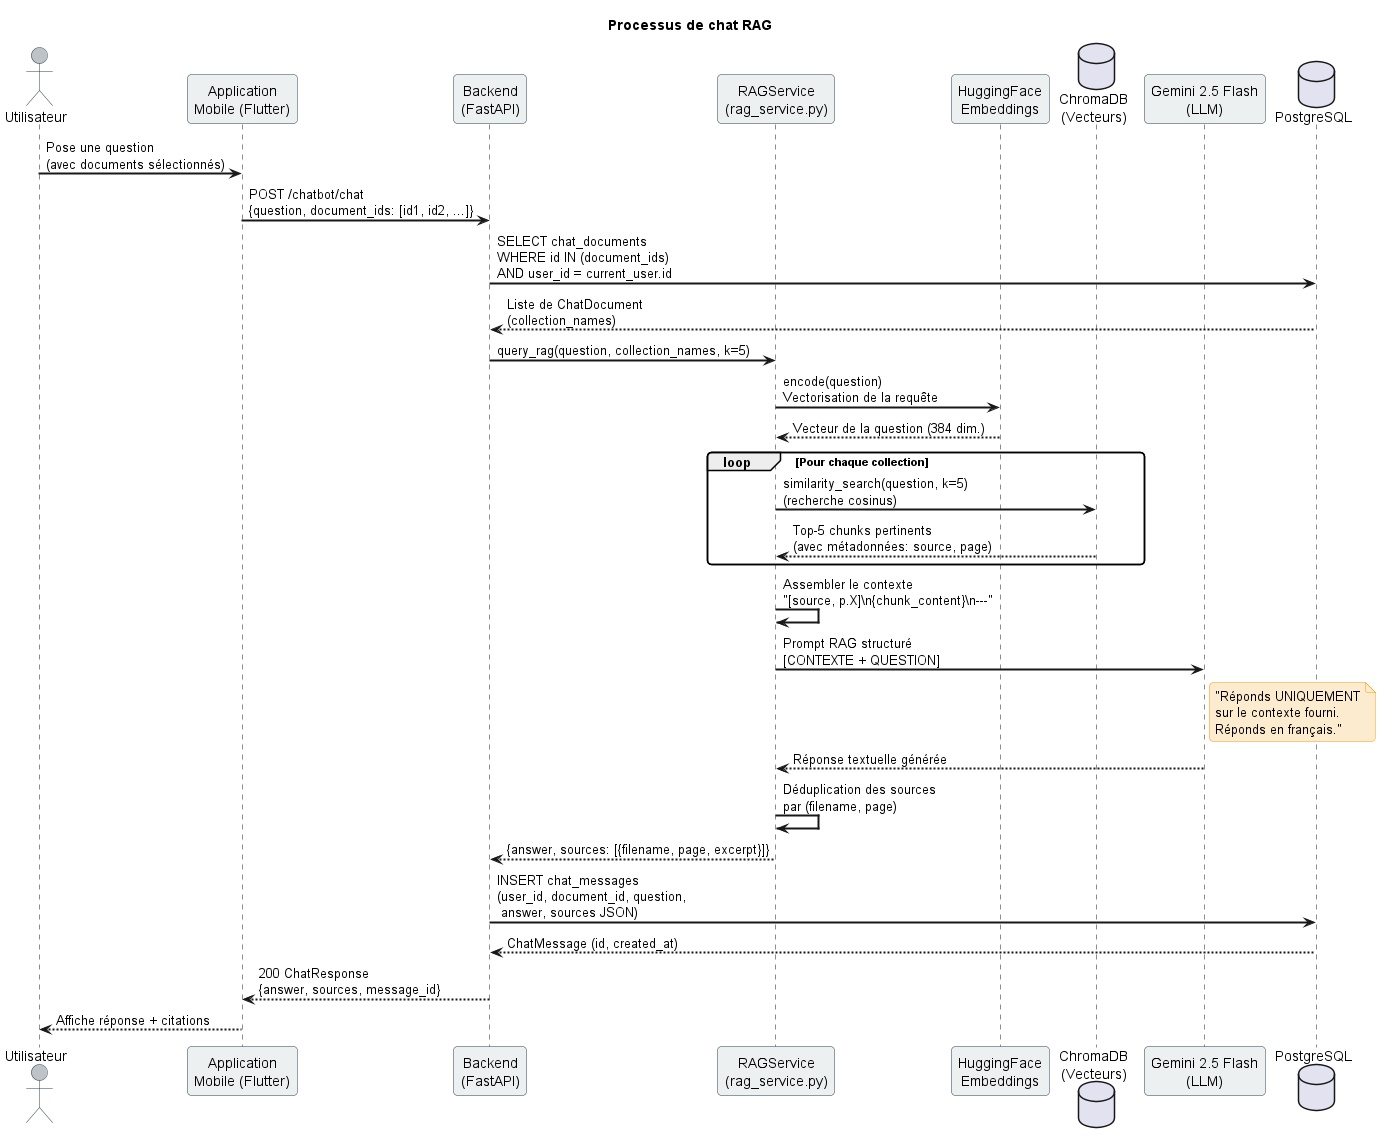
\includegraphics[width=0.85\textwidth]{images/seq_chat_rag.jpg}
\caption{Diagramme de séquence du processus de chat RAG}
\label{fig:seq_chat_rag}
\end{figure}

%----------------------------------------
\subsubsection{Processus de génération de quiz}

Le processus de génération de quiz exploite le contenu des documents indexés pour produire des questions à choix multiples. Comme illustré dans la Figure~\ref{fig:seq_quiz}, le backend récupère un échantillon diversifié de chunks, construit un prompt spécialisé et envoie la requête à Groq. Le résultat JSON est validé avant d'être persisté en base de données.

\begin{figure}[H]
\centering
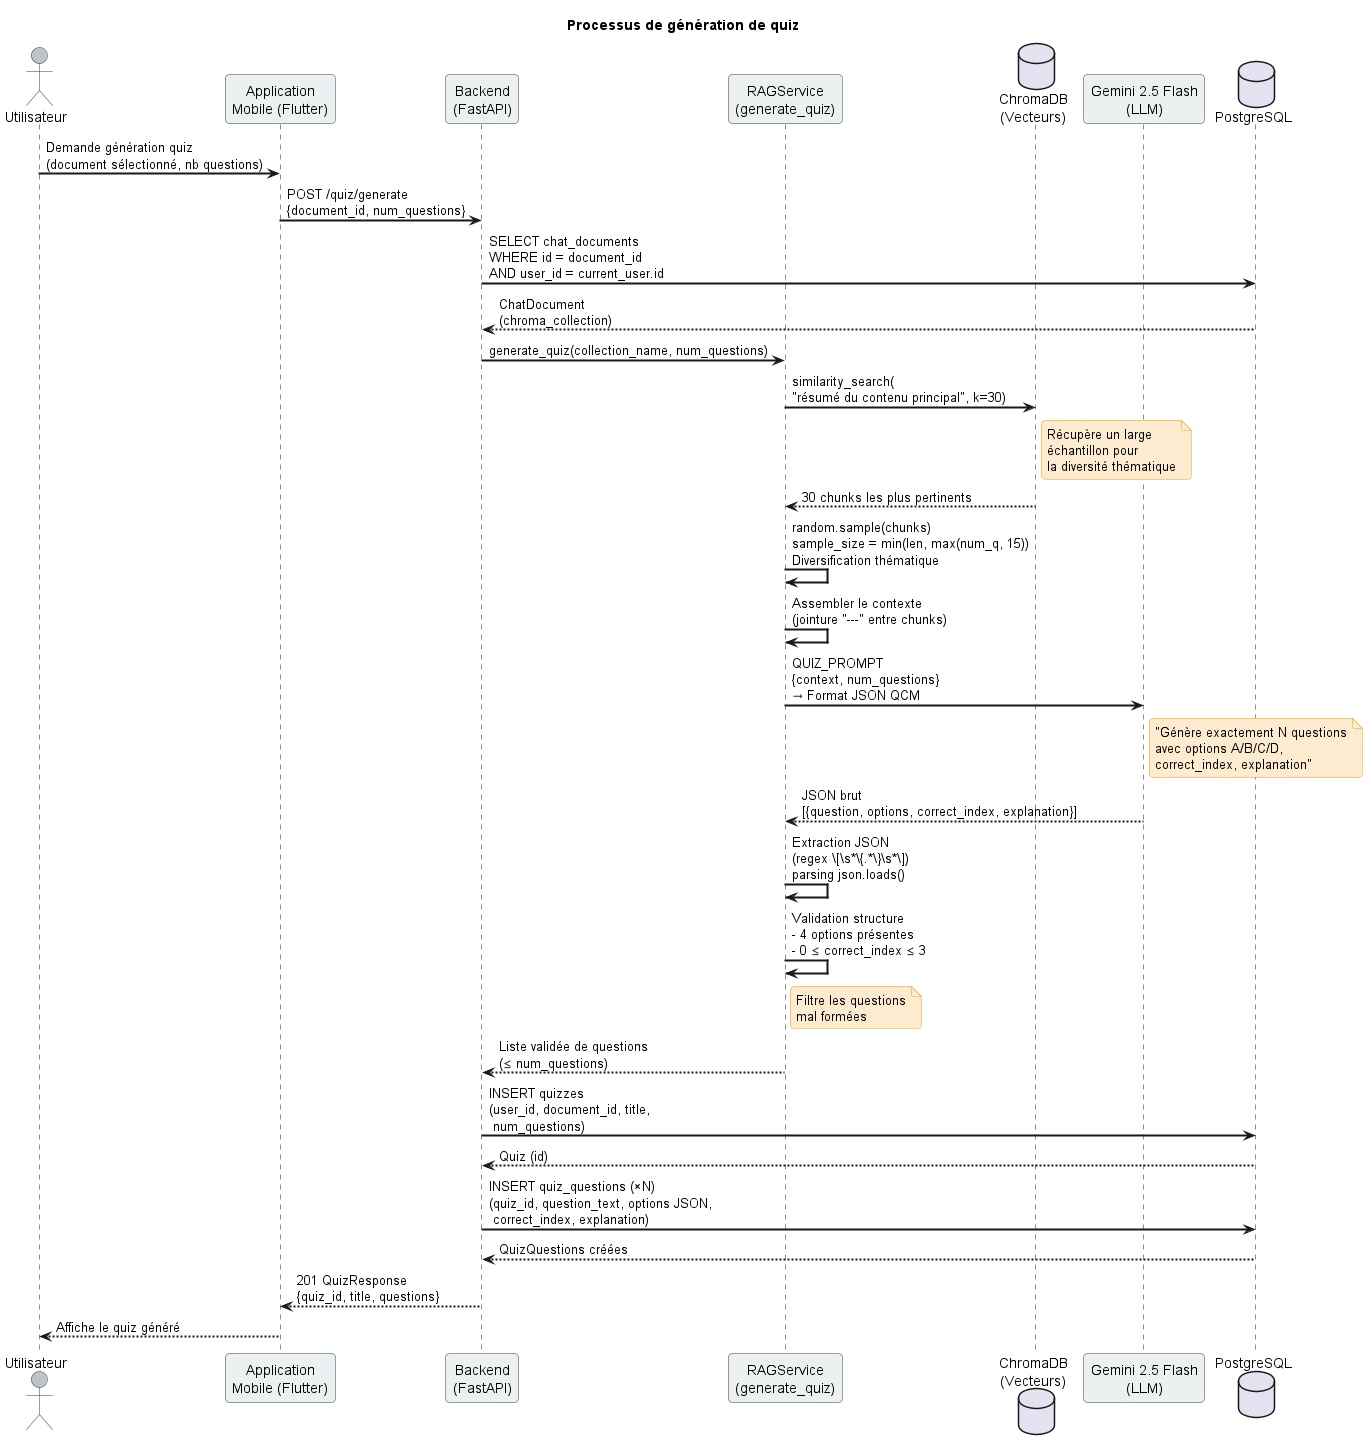
\includegraphics[width=0.85\textwidth]{images/seq_quiz.jpg}
\caption{Diagramme de séquence de la génération de quiz}
\label{fig:seq_quiz}
\end{figure}

%----------------------------------------
\subsubsection{Processus de génération du planning intelligent}

Le processus de planification combine un calcul algorithmique avec l'intelligence artificielle. Comme illustré dans la Figure~\ref{fig:seq_planning}, le backend détermine d'abord les créneaux libres de manière déterministe, puis demande à Groq d'assigner des sujets pertinents à chaque créneau. En cas d'échec de l'IA, un mécanisme de fallback garantit la production d'un planning valide.

\begin{figure}[H]
\centering
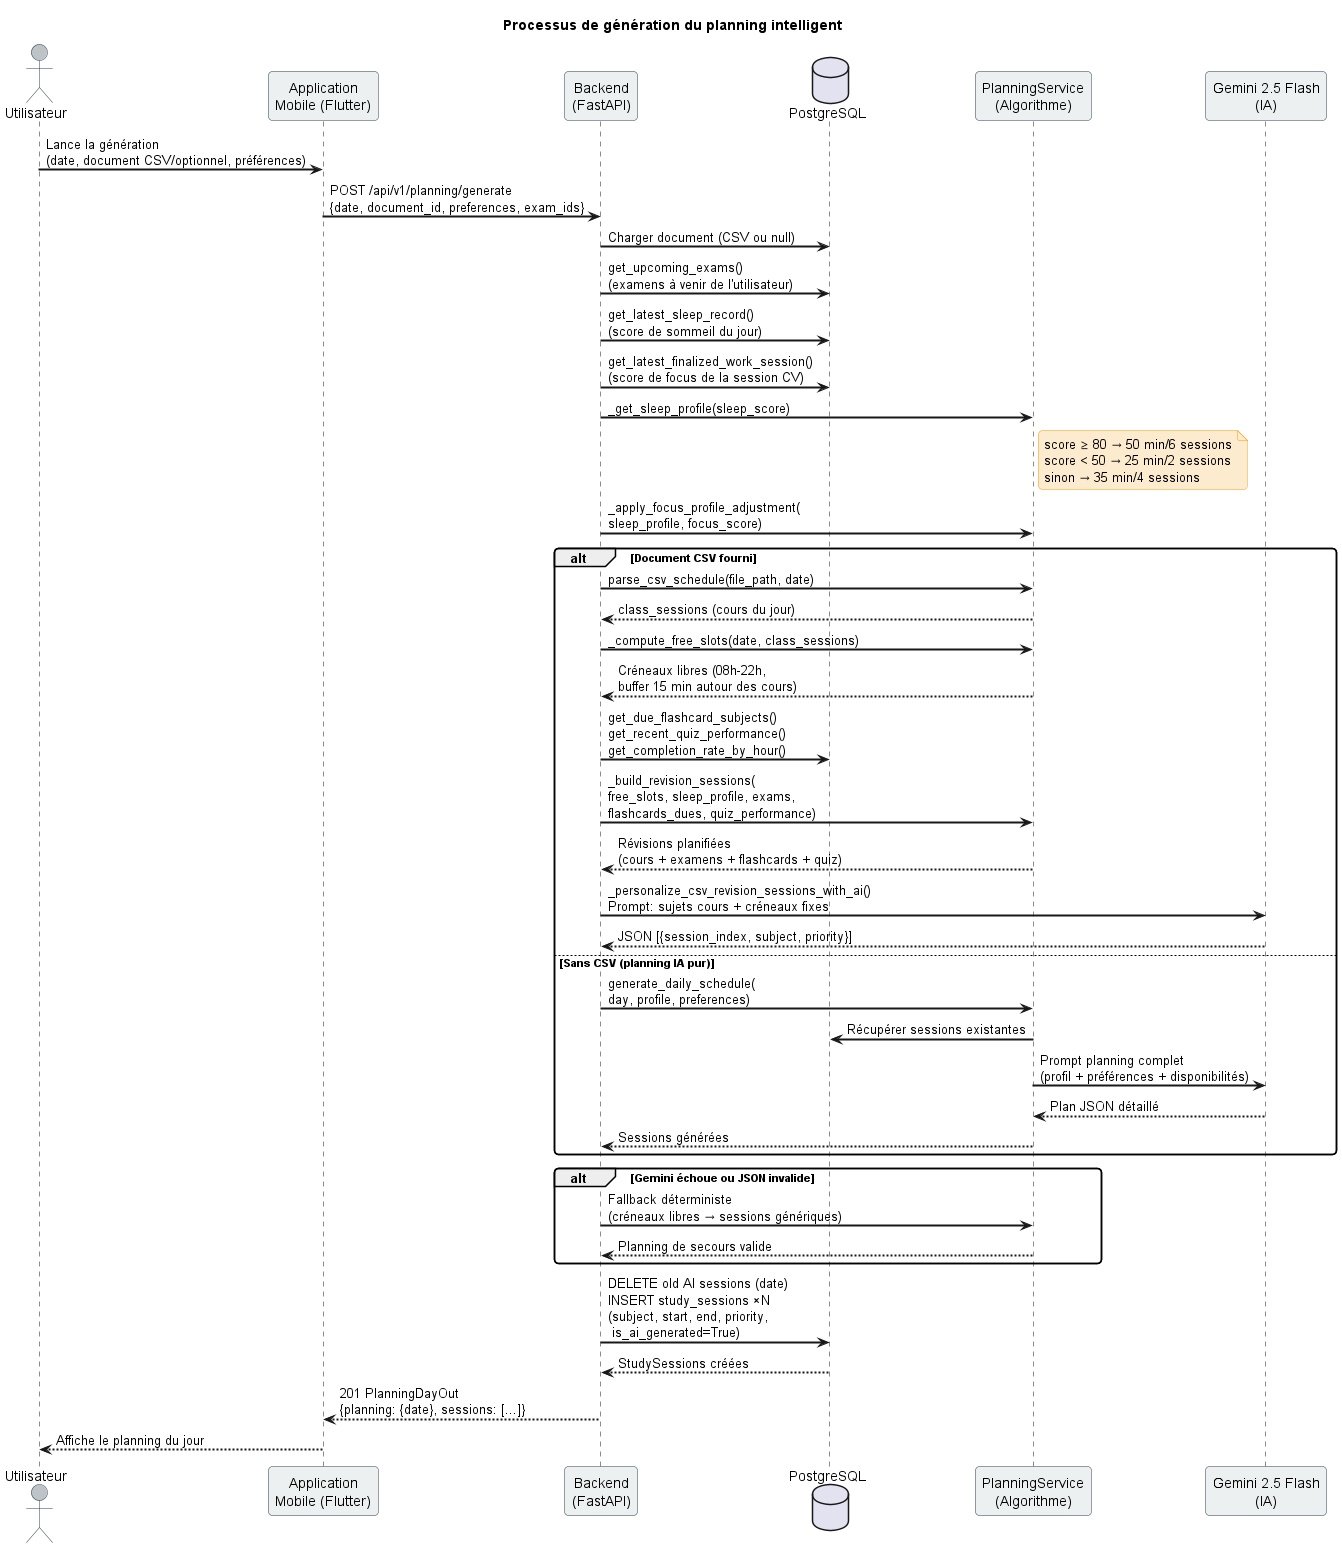
\includegraphics[width=0.85\textwidth]{images/seq_planning.jpg}
\caption{Diagramme de séquence de la génération du planning intelligent}
\label{fig:seq_planning}
\end{figure}


\subsection{Diagramme de classes du Sprint 3}

Le diagramme de classes présenté dans la Figure~\ref{fig:class_sprint3} décrit la structure des modules développés durant ce sprint.

La classe \textit{ChatDocument} représente un document importé et est associée aux messages du chatbot (\textit{ChatMessage}), aux quiz (\textit{Quiz}) et aux flashcards (\textit{Flashcard}). La classe \textit{Quiz} contient une liste de \textit{QuizQuestion}, chacune disposant d'options et d'une correction.

La classe \textit{Flashcard} intègre les paramètres de l'algorithme SM-2 (ease\_factor, interval, repetitions, next\_review). La classe \textit{StudySession} représente une session de planning avec son sujet, ses horaires et son statut.

Les services \textit{RAGService}, \textit{PlanningService} et \textit{SM2Service} centralisent respectivement les opérations de recherche sémantique, de planification et de répétition espacée.

\begin{figure}[H]
\centering
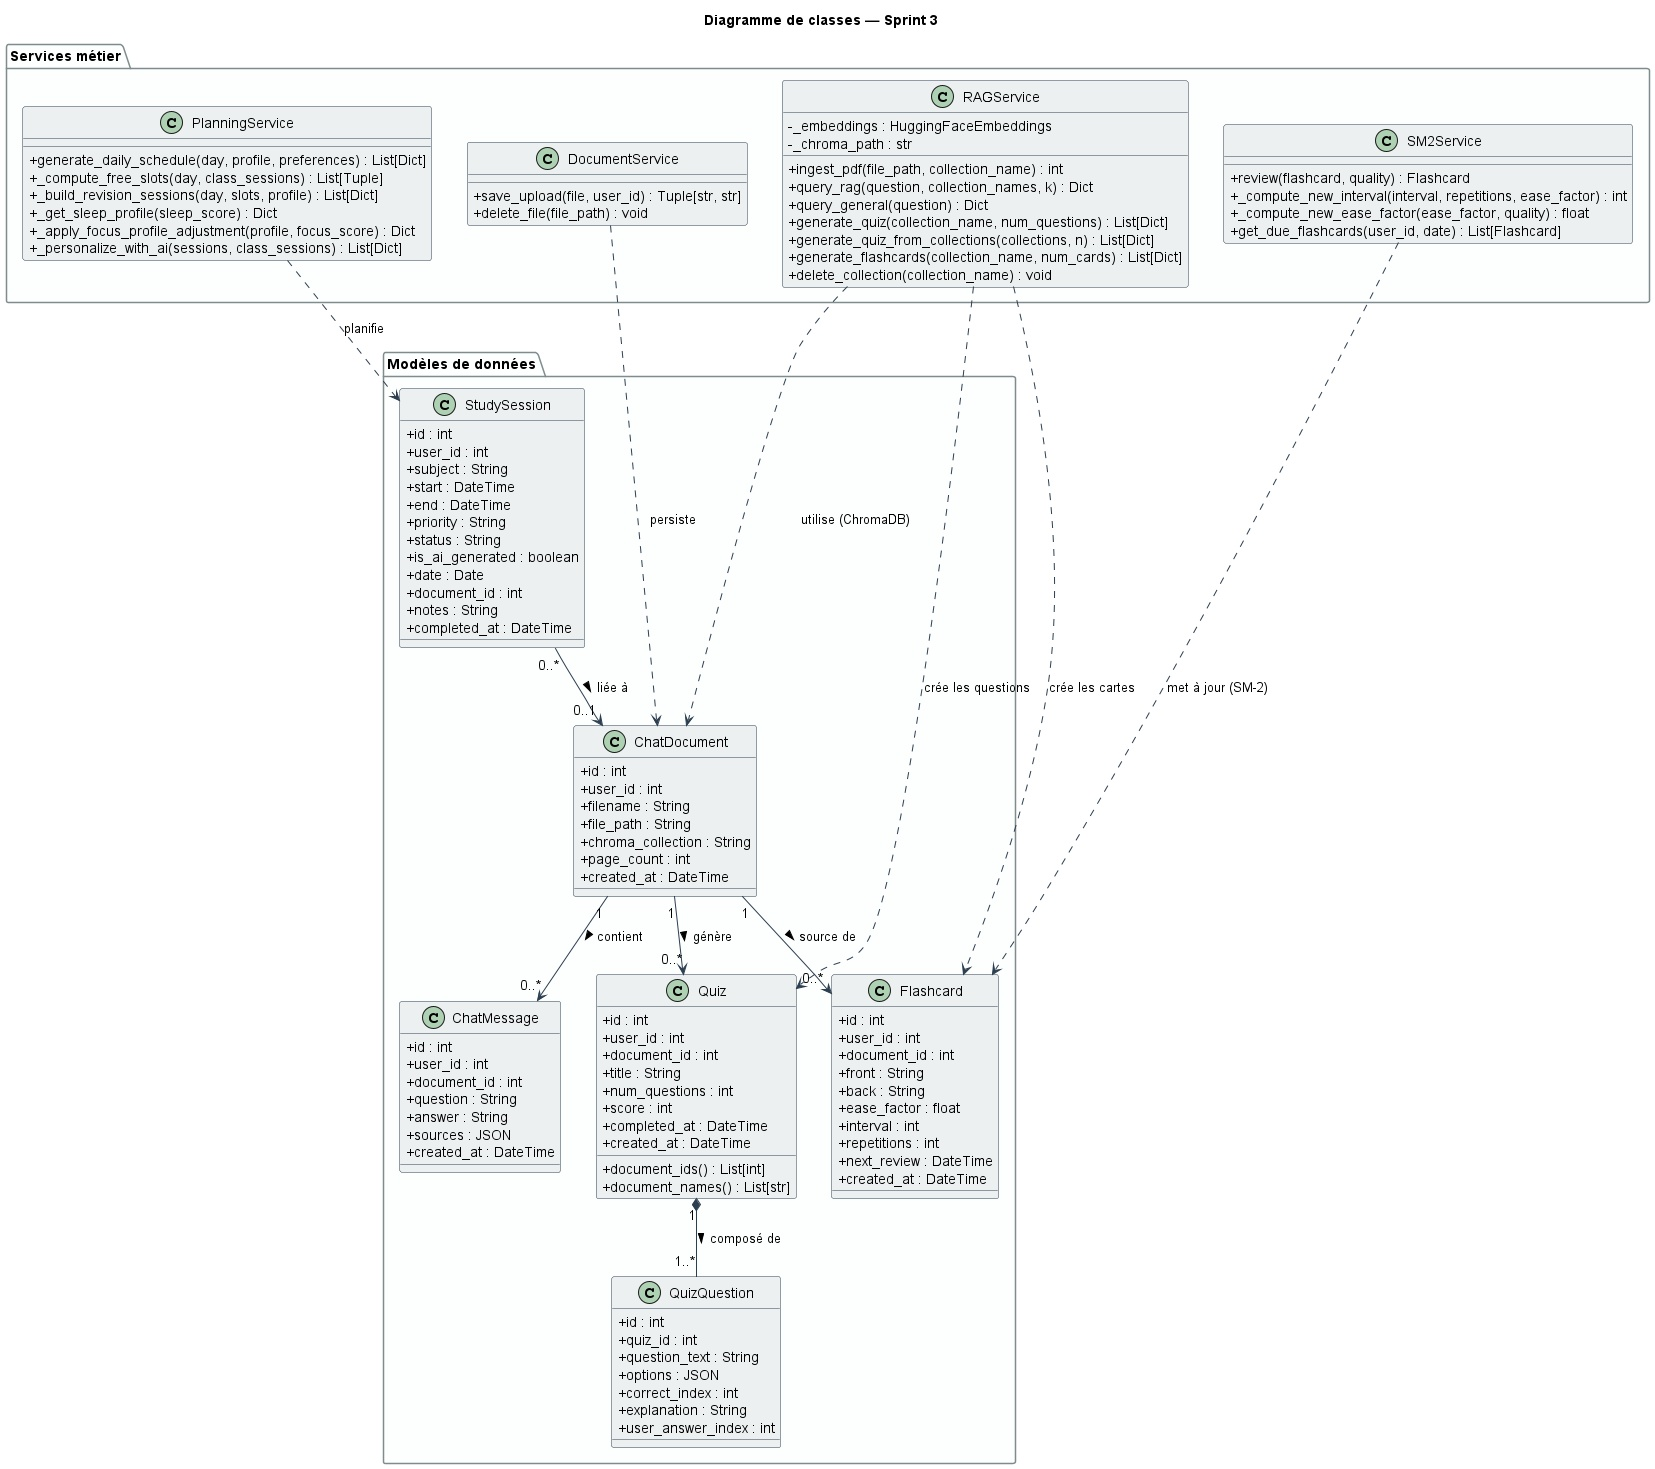
\includegraphics[width=0.85\textwidth]{images/class_sprint3.jpg}
\caption{Diagramme de classes du Sprint 3}
\label{fig:class_sprint3}
\end{figure}

%%%%%%%%%%%%%%%%%%%%%%%%%%%%%%%%%%%%%%%%%%%%%%%%%%%%%%%%%%%%%%%%
\section{Implémentation}

Cette section présente les principales interfaces développées dans le cadre du Sprint 3. Elles illustrent les fonctionnalités liées au chatbot RAG, à la génération de quiz et de flashcards, ainsi qu'à la planification intelligente.

%--------------------------------------

\subsection{Interfaces de l'application mobile}

Les interfaces développées dans le cadre du Sprint 3 permettent à l'utilisateur d'interagir avec les modules d'intelligence artificielle du système. Elles couvrent l'assistant pédagogique, les outils de révision et le planning adaptatif.

%----------------------------------------
\subsubsection{Interface du chatbot RAG}

L'interface du chatbot permet à l'utilisateur de poser des questions sur ses documents importés et d'obtenir des réponses contextualisées. Elle offre également la possibilité de sélectionner les documents sources et de consulter l'historique des échanges.

\begin{figure}[H]
\centering
\includegraphics[width=0.35\textwidth]{images/chatbot1.jpg}
\hspace{0.5cm}
\includegraphics[width=0.35\textwidth]{images/chatbot2.jpg}
\caption{Interface du chatbot RAG : gestion des documents et conversation}
\label{fig:chatbot_screens}
\end{figure}

%----------------------------------------
\subsubsection{Interfaces de génération et passage de quiz}

Ces interfaces permettent à l'utilisateur de générer des quiz QCM à partir de ses documents, de répondre aux questions et de consulter les résultats détaillés avec explications.

\begin{figure}[H]
\centering
\includegraphics[width=0.35\textwidth]{images/quiz1.jpg}
\hspace{0.5cm}
\includegraphics[width=0.35\textwidth]{images/quiz2.jpg}
\caption{Interfaces de quiz : génération et passage du quiz}
\label{fig:quiz_screens}
\end{figure}

%----------------------------------------
\subsubsection{Interfaces des flashcards avec révision espacée}

Les interfaces de flashcards permettent à l'utilisateur de générer des cartes de révision, de les parcourir et d'évaluer sa qualité de rappel. Le système utilise l'algorithme SM-2 pour planifier automatiquement les prochaines sessions de révision.

\begin{figure}[H]
\centering
\includegraphics[width=0.35\textwidth]{images/flashcard1.jpg}
\hspace{0.5cm}
\includegraphics[width=0.35\textwidth]{images/flashcard2.jpg}
\caption{Interfaces des flashcards : génération et révision}
\label{fig:flashcard_screens}
\end{figure}

%----------------------------------------
\subsubsection{Interface du planning intelligent}

L'interface de planning affiche les sessions d'étude générées automatiquement par le système. L'utilisateur peut consulter son planning quotidien ou hebdomadaire, créer des sessions manuellement, et visualiser l'adaptation des créneaux en fonction de son état de sommeil et de ses examens.

\begin{figure}[H]
\centering
\includegraphics[width=0.35\textwidth]{images/planning1.jpg}
\hspace{0.5cm}
\includegraphics[width=0.35\textwidth]{images/planning2.jpg}
\caption{Interface du planning intelligent : vue quotidienne et génération IA}
\label{fig:planning_screens}
\end{figure}

%%%%%%%%%%%%%%%%%%%%%%%%%%%%%%%%%%%%%%%%%%%%%%%%%%%%%%%%%%%%%%%

\section{Conclusion}
\addcontentsline{toc}{section}{Conclusion}

Ce troisième sprint a permis de mettre en place les modules d'intelligence artificielle au cœur du système \textit{Smart Focus}. Le chatbot RAG, les quiz QCM, les flashcards avec révision espacée SM-2 et le planning intelligent constituent désormais un ensemble cohérent d'outils pédagogiques.

L'architecture adoptée, combinant un calcul déterministe des créneaux avec une personnalisation par IA via Groq, garantit à la fois la fiabilité et la pertinence des résultats produits. Ces fonctionnalités posent les bases pour l'intégration du monitoring temps réel et des alertes intelligentes dans le sprint suivant.
